%%%%%%%%%%%%%%%%%%%%%%%%%%  phdsymp_sample2e.tex %%%%%%%%%%%%%%%%%%%%%%%%%%%%%%
%% changes for phdsymp.cls marked with !PN
%% except all occ. of phdsymp.sty changed phdsymp.cls
%%%%%%%%%%                                                       %%%%%%%%%%%%%
%%%%%%%%%%    More information: see the header of phdsymp.cls   %%%%%%%%%%%%%
%%%%%%%%%%                                                       %%%%%%%%%%%%%
%%%%%%%%%%%%%%%%%%%%%%%%%%%%%%%%%%%%%%%%%%%%%%%%%%%%%%%%%%%%%%%%%%%%%%%%%%%%%%%


%\documentclass[10pt]{phdsymp} %!PN
\documentclass[twocolumn]{phdsymp} %!PN
%\documentclass[12pt,draft]{phdsymp} %!PN
%\documentstyle[twocolumn]{phdsymp}
%\documentstyle[12pt,twoside,draft]{phdsymp}
%\documentstyle[9pt,twocolumn,technote,twoside]{phdsymp}

\usepackage[english]{babel}       % Voor nederlandstalige hyphenatie (woordsplitsing)

\usepackage{graphicx}			% Om figuren te verwerken.
\graphicspath{{../../../images/}}
\usepackage{booktabs}
\usepackage{times}
\usepackage{siunitx}
\usepackage{xcolor}

\hyphenation{si-mu-la-ted re-a-lis-tic packets really in-clu-ding}

\def\BibTeX{{\rm B\kern-.05em{\sc i\kern-.025em b}\kern-.08em
    T\kern-.1667em\lower.7ex\hbox{E}\kern-.125emX}}

\newtheorem{theorem}{Theorem}

\begin{document}

\title{Evaluating Human Electromagnetic Exposure in a UAV-aided Network}

\author{Thomas Detemmerman}

\supervisor{Wout Joseph, Luc Martens, Luc Martens, German Dario Castellanos Tache}

\maketitle

\begin{abstract}
Society relies more than ever on the availability of the wireless networks but is at the same time also 
concerned about the potential health effects of the electromagnetic radiation caused by these networks.
The government has enforced strict legislations to which mobile devices and base stations have to satisfy.

This research investigates the specific absorption rate caused by these electromagnetic waves by taking all mobile devices and base stations into account.
To accomplish this goal, the deployment tool developed by the WAVES research group at Ghent University will be used. This tool simulates an entire network 
where transmission towers are represented by femtocell base stations attached to drones. This research also investigates how these drones can be guided 
in order to reach certain goals like minimizing power consumption or electromagnetic exposure.

It looks from the results that ... (todo)
\end{abstract}

\begin{keywords}
LTE, Electromagnetic Radiation, power consumption, drones, femtocell, microstrip patch antenna, radiation pattern, specific absorption rate (SAR)
\end{keywords}

\section{Introduction}
\PARstart{S}{ociety} is constantly getting more and more dependent on wireless communication. On any
given moment, in any given location, an electronic device can request to connect to the bigger
network. Devices need more than ever to be connected. Also in exceptional and possibly life-threatening situations, the public relies on the cellular
network. For example during the terrorist attacks at Brussels Airport, mobile network operators
saw all telecommunications drastically increasing causing moments of contention. Some
operators decided to temporarily exceed the exposure limits in order to handle all connections.
Electromagnetic exposure can however not be neglected. Research shows how excessive electromagnetic
radiation can cause diverse biological side effects [3].
This research tries to map  the electromagnetic exposure of the average user. In order 
for this to work, an existing planning tool is used and the
three prominent sources of radiation in a telecommunication network are investigated, being: the user’s own
phone, all base stations and all devices from other users in the network.
The electromagnetic behaviour of the network will be analysed by applying the tool in different
scenarios to give insight which variables influence the exposure and how the network can be
optimized accordingly.



\section{State of the Art}
\subsection{Electromagnetic exposure}

Users in a telecommunication network are exposed to various sources of electromagnetic radiation, being:
the user's own phone,
 the base station that is serving this user, 
all devices from other users in the network and all 
other active base stations that are not serving this user. Thi. 
This electromagnetic exposure is expressed in $V/m$. Once this exposure is absorbed by the human 
body we speak of specific absorption rate (SAR) and is expressed in $W/kg$. All these values are 
subjected to limitations enforced by the government. This research is done in Ghent, 
a Flamish city in Belgium, where in the 2.6 GHz frequency band, an individual antenna cannot exceed 4.5 V/m and the cumulative sum of all 
fixed sources has its maximum at 31 V/m \cite{J23, S13_normenBelgie}. The maximum SAR-values have been 
defined at $SAR_{10g}$ for a whole body SAR and $2 W/kg$ for localized $SAR_{10g}$ at head and torso area \cite{J30}. 

Several papers calculate exposure originating from certain sources  \cite{J6_originalExposureFormula, J1, J10_RDP, J10.1}. 
where some convert the UL radiation into localized specific absorption rates \cite{ J10_RDP, J10.1}. 
With the advent of 5G, paper \cite{J17_kuehn2019modelling} describes 
how localized SAR values are achieved different sources
Finally, \cite{J22_plets2015joint} describes how both UL and DL traffic can be converted into a single  whole body SAR values.

In a realistic network, some users are calling while others are using other types of telecommunication services like browsing the web.
Therefore, all absorbed electromagnetic exposure should be expressed in whole body SAR while still covering all sources.

\subsection{Optimized UAV-aided networks}

A UAV knows several applications. It was originally mainly used to support the military for surveillance and remote attacks without 
endangering pilots \cite{U12}. However, UAVs have recently become more accessible by the general public due to decreasing costs. This 
allowed UAVs to be researched for various applications.

A UAV equipped with a femtocell base station antenna will be called a UABS
which brings several advantages like like mobility and rapid deployment. 
However, it brings also challenges like limited weight of the payload and sparse power supply.

Kawamoto et al. introduced in \cite{U11} a WiFi network with the support of  UAVs while considering resource allocation 
and antenna directivity. 
Gangula et al. illustrates in \cite{U10} how UAVs can be  used as a relay for LTE. 
Zeng et al. proposes in  \cite{U12} a tutorial in 5G-and-beyond wireless systems where challenges like 
energy consumption, mobility and antenna direction are discussed. 

Mozaffari et al. provides in \cite{U3} guidelines on how to optimize and analyse UAVs equipped for 
wireless communication equipment. Issues like deployment, performance and power consumption are addressed.
One path that has been excessively researched are location optimization solutions where the network is 
designed in such a way that certain goals are achieved \cite{U6,U7,U8,U9}.
These optimizations can be achieved through different implementation methods like heuristic algorithms \cite{U3,U5}.

Optimizing the network towards electromagnetic exposure is rather limited.
Deruyck et al. discusses in \cite{J1} how the terrestrial network can be optimized towards either a minimal exposure or minimal power consumption of the entire network.
However, to the best of the author knowledge, no research has been done where a UABS-network have been optimized towards electromagnetic exposure.

\subsection{Technologies}

For the deployment of the network, the more robust UAVs from \cite{J2} will be used. The UABSs will operate in the 2.6 Ghz 
bandwidth. Since the users are assumed to experience a constant electromagnetic exposure without interruptions frequency division duplex is used.

% problem antennae on drones
The onboard antenna of the UAV will act as the gateway between the UE and the backhaul network.
However, determining which antenna to use and how to position it, can be challenging.
The radiation pattern from the antenna can be influenced by the UAV \cite{A1}.
Also the fact that the UAV will hover above the user makes tradional 2D modelling insufficient
A 3D-model which accounts for both elevation and azimuth directivity 
will be required \cite{U12}.

The easiest radiation pattern is a hypothetical isotropic radiator which radiates equally in all directions.
Antennae that radiate equal quantities for a certain plane  are called omnidirectional antennae \cite{U12} and several types 
exist. Different type of omnidirectional antennae like monopoles, dipoles and wing antennae 
have been considered \cite{A4,A10,A11,A12}.

Another type of antennae are directional antennae, more precisly microstrirp patch antenna 
in various configurations have been a point of interesset \cite{A5,A6,A8}.
since they provide several advantages compared to traditional antennae \cite{J13_microstripadvantages, J14_antennadesign}
like lightweightness, low in cost and thin causing them to be more aerodynamic. 

A basic microstrip antenna like figure \ref{fig:basicpatchantenna} consists of a ground plane and
a radiating patch, both separated with a dielectric substrate. 
Several variations exist like microstrip patch antenna, microstrip slot antenna and printed dipole antenna which
all have similar characteristics \cite{J13_microstripadvantages, J14_antennadesign}. They are all thin, support dual frequency operation and they all have the disadvantage that they 
will transmit at frequencies outside the aimed band which is also known as
spurious radiation. The microstrip patch and slot antenna support both linear
and circular polarization while the printed dipole only supports linear polarization. Further is the fabrication of a microstrip patch antenna considered to be the easiest of the considered patch antennae \cite{J13_microstripadvantages}. 


\section{Scenario's}

The default configuration is given below and is always applicable unless mentioned otherrwise. 

\begin{table}[!htb]
\centering
\begin{tabular}[t]{ll}
        \toprule
        \multicolumn{2}{l}{\textbf{Broadband cellular network}} \\
        \hline
        \hspace{3mm}  technology        & LTE     \\
        \hspace{3mm}  frequency         & 2.6 GHz \\
        \hline
        \multicolumn{2}{l}{\textbf{Carrier}} \\
        \hline  
        \hspace{3mm}  carrier power        & 13.0 A   \\
        \hspace{3mm}  average carrier speed        & 12.0 m/s \\
        \hspace{3mm}  average carrier power usage      & 17.33 Ah    \\
        \hspace{3mm}  carrier battery voltage       & 22.2 V \\
        \hline
        \multicolumn{2}{l}{\textbf{Femtocell antenna}} \\
        \hline  
        \hspace{3mm}  maximum $P_{tx}$          & 33 dBm   \\
        \hspace{3mm}  antenna  direction        & downwards (az: \ang{0}; el: \ang{90})    \\ 
        \hspace{3mm}  gain                      & 4 dBm   \\ 
        \hspace{3mm}  feeder loss               & 2 dBm   \\ 
        \hspace{3mm}  implementation loss       & 0 dBm   \\
        \hspace{3mm}  radiation pattern         & EIRP or microstrip patch\\
        \hspace{3mm}  height                    & 100m  \\
        \hline
        \multicolumn{2}{l}{\textbf{UE Antenna}} \\
        \hline 
        \hspace{3mm} height                     & 1.5m from the floor       \\ 
        \hspace{3mm} gain                      & 0 dBm   \\ 
        \hspace{3mm} feeder loss               & 0 dBm   \\ 
        \hspace{3mm} radiation pattern         & EIRP  \\
        \hspace{3mm} number present in the network         & 224  \\
        \toprule
\end{tabular}
\caption{Overview of default configuration values.}
\end{table}


Four possible configurations  will be investigated in different scenarios. Their are two possible antennae, namely EIRP 
and microstrip pach antenna which can both be applied in a power consumption optimized network or an exposure optimized network.
\textcolor{red}{configuraiton matrix??}

Three main scenarios will be investigated. 
First, only one user with one drone will be present in the network. SAR, electromagnetic exposure, power consumption 
and antenna transmission power are investigated.

In a second scenario, the network is expanded for multiple users but with still only one drone available. 
The scenario is divided into two cases. One with a variable flying height but with a fixed 
number of 224 users which is an average day 
at 5 p.m. in Ghent. In the other case, the number of users varies but the flying height is set to 100. 
\textcolor{red}{Todo: bronnen 100m and 224 users}. The power consumption, electromagnetic exposure and specific 
absorption rate are investigated in four different configurations.

The third scenario is quite similar then the previous scenario with the same 
two cases with each four configurations. The only exception is that an unlimited number of UABSs are available.

\section{Methodology}
\subsection{Electromagnetic Exposure}
\subsection{Microstrip Pach antenna}
A microstrip patch antenna is chosen because it allows easy production but more important, it has a low weight 
and has a thin profile causing it to be very aerodynamic which is useful when attaching it to a drone \cite{J13_microstripadvantages}.

The dimensions of the antenna depend on the frequency it is operating at and the characteristics of the used substrate.
The antenna will be radiating at a center frequency $f_0$ of 2.6 GHz. Each substrate has a dielectric constant $\epsilon_r$ representing 
the permittivity of the substrate and depends on the used material.
Substrates with a high dielectric constant and low height 
reduce the dimensions of the antenna
while a lower dielectric constant with a high height improves antenna performance. 
In this document, a substrate like glass 
is chosen because of the higher dielectric constant of $\epsilon_r = 4.4$ compared to materials like teflon with only a dielectric 
constant of $\epsilon_r = 2.2$ \cite{J14_antennadesign}. 
Doing this in combination with an antenna height of 2.87 mm will decrease the dimensions of the entire antenna surface.
This comes in handy since drones only have limited space available.

\begin{table}[h!]
\centering
\begin{tabular}{|l|c|l|}
\hline
 description            & symbol          & value         \\    \hline
 center frequency       & $f_0$           & 2600 Hz       \\ 
 dielectric constant    & $\epsilon_r$    & 4.4         \\ 
 heigt of the substrate & $h$             & 0.00287 m    \\ \hline
\end{tabular}
\caption{Overview of configuration parameters.}
\label{table:antennaparas}
\end{table}

The dimensions of the radiating patch can be calculated with the formulas from \cite{J14_antennadesign} and \cite{J15_antennadesign}.
Doing so result in a radiating patch of 35.09 mm by 26.55 mm and a groundplane of at least 52.40 mm by 43.80 mm.

\begin{figure}[h!]
\centering
  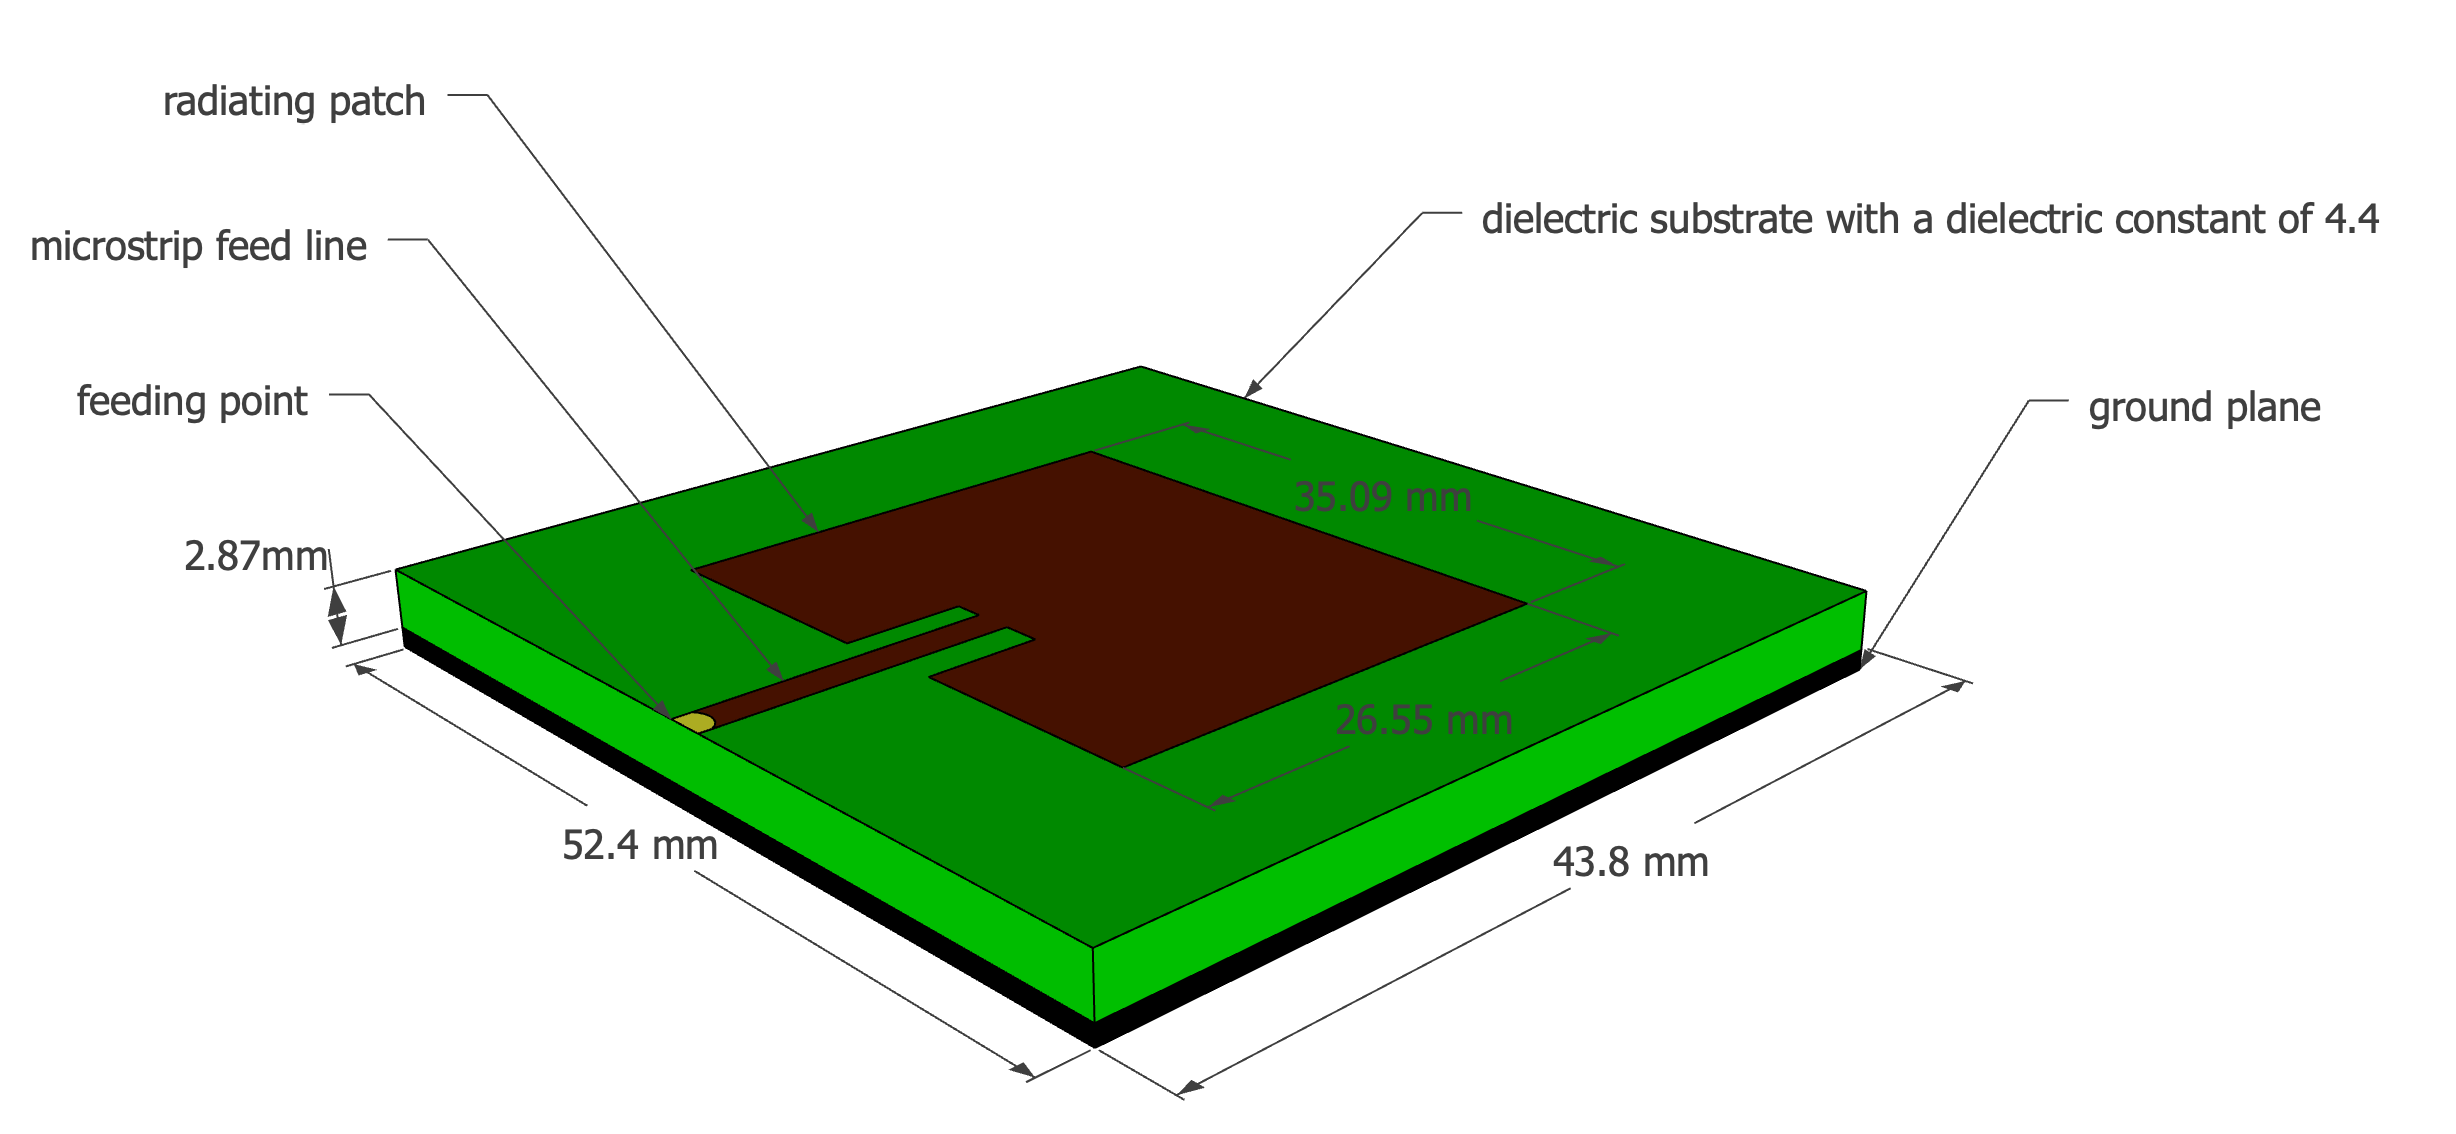
\includegraphics[width=\linewidth]{MicrostripAntenna.png}
  \caption{Design of the microstrip patch antenna.}
  \label{fig:basicpatchantenna}
\end{figure}

This corresponds to the following radiation pattern 

\begin{figure}[!htb]
\minipage{0.49\textwidth}
  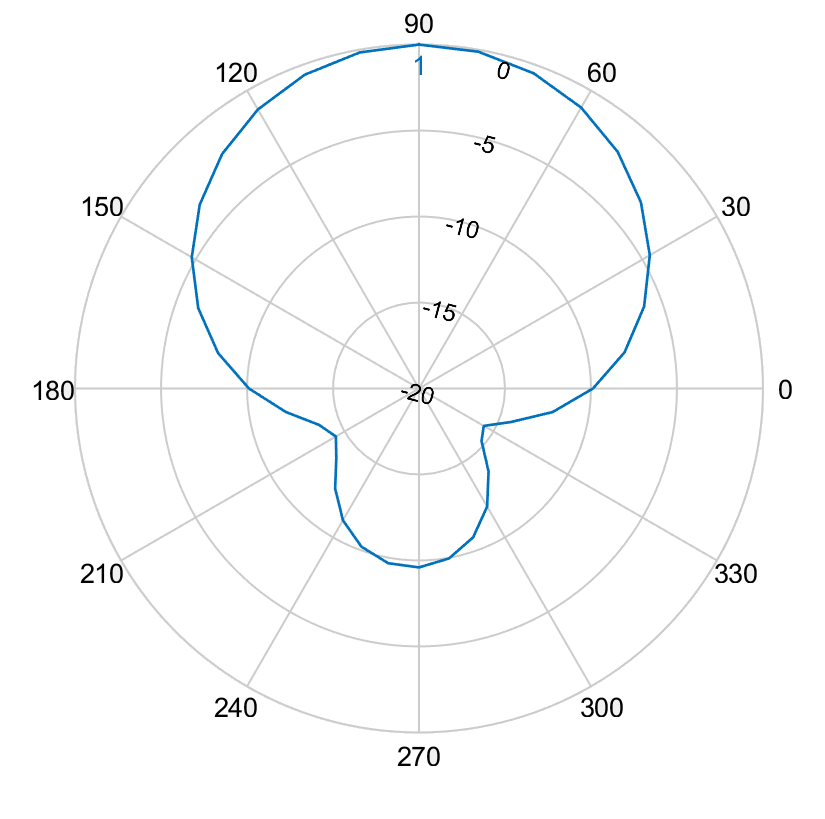
\includegraphics[width=\linewidth]{pattern2/ep.png} 
\endminipage\hfill
\minipage{0.49\textwidth}%
  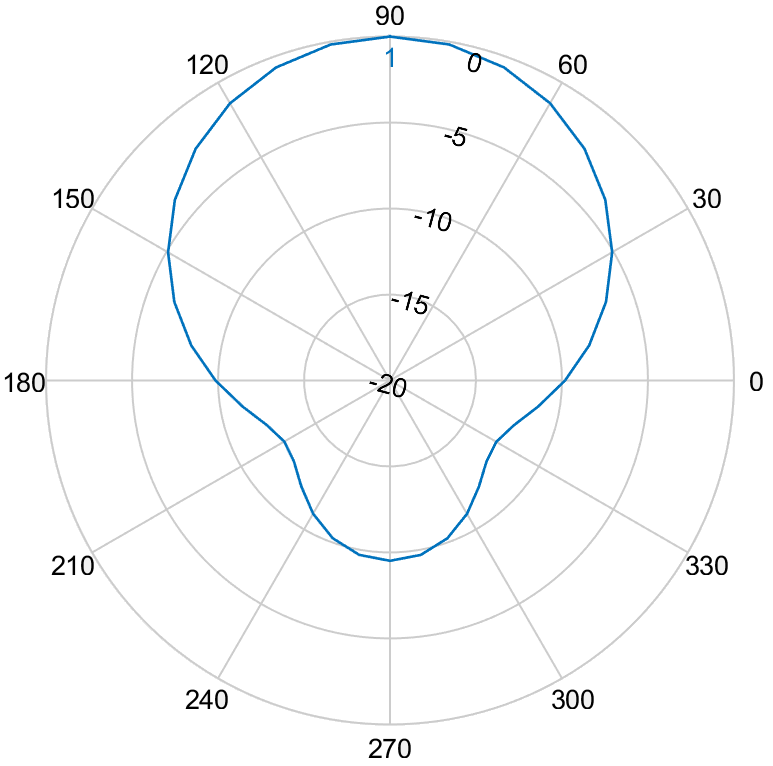
\includegraphics[width=\linewidth]{pattern2/hp.png}
\endminipage
  \caption{Radiation pattern 1: On the left a 3D model of the entire pattern with the configuration as described above. In the middle a 2D radiation pattern of the E-plane and at the right a 2D model of the H-plane.}
\end{figure}

\subsection{Optimizing the network}

Margot et al. discusses in \cite{J1} how a terrestrial  telecommunication network eighter can  be optimized towards electromagnetic 
exposure of an individual or towards power consumption of the entire network. 
However an increasing transmission power of an antenna comes with an increasing electromagnetic exposure. This is not the case considering
both values for an entire network. In fact, the authors from   prove that both become inversely equivalent.
The reason the network behaves like this is because it is often cheaper to increase the exposure of an already active base station 
then activating a new one. 
This lead to the following fitness function which is based on \cite{J1}.

\begin{equation} 
f = w * \left(1 - \frac{E_m}{E_{max}}\right) + (1 - w)*\left(1 - \frac{P}{P_{max}}\right) * 100
\label{eq:fitnessfunction}
\end{equation}

Formula \ref{eq:fitnessfunction} returns a fitness value which represents the performance of the entire network. 
$w$ is the importance factor of electromagnetic exposure ranging from 0 to 1, boundaries included. A $w$ set to zero means that electromagnetic 
exposure is not important. Such a network will therefore be called a power consumption optimized network. 
Likewise, a $w$ set to one means that minimizing exposure is top priority and will result in an exposure optimized  network. $P_{max}$ is the power consumption of all UABSs, both active and inactive, when radiating at the highest possible level 
while $P$ is the effective power used by the current designed network. 
This will be the power required for the flying drones themselves and their antenna.
$E_m$ will be the weighted exposure of the average user for the current designed network and $E_{max}$ the weighted average electromagnetic exposure when all antennae are at their highest power level.

When optimizing the network, it is not only important to consider the average exposure of all users, but also to limit high extremes \cite{J1}. A weighted average 
will be used not only considering the median but also the 95 percentile from all users' DL exposure using formula \ref{eq:em}. 
Since both values are considered to have equal importance, the weight factors $w_1$ and $w_2$ will both have an equal importance of 50\%. 

\begin{equation} 
E_m = \frac{w_1 * E_{50} + w_2 * E_{95}}{w_1 + w_2}
\label{eq:em}
\end{equation}







\section{Resultaten}
todo

\section{Conclusie}
todo

\section{Acknowledgement}
Special thanks to the WAVES research group at Ghent University for providing 
access to their capacity based deployment tool and therefore making this research possible.

\subsection{Referencies}
todo


\nocite{*}
\bibliographystyle{phdsymp}
%%%%%\bibliography{bib-file}  % commented if *.bbl file included, as
%%%%%see below


%%%%%%%%%%%%%%%%% BIBLIOGRAPHY IN THE LaTeX file !!!!! %%%%%%%%%%%%%%%%%%%%%%%%
%% This is nothing else than the phdsymp_sample2e.bbl file that you would%%
%% obtain with BibTeX: you do not need to send around the *.bbl file        
%%
%%---------------------------------------------------------------------------%%
%
\begin{thebibliography}{1}
\bibitem{paper}
Bart Lannoo, Didier Colle, Mario Pickavet, Piet Demeester,
\newblock {\em Optical Switching Architecture to Implement Moveable Cells in a Multimedia Train Environment},
\newblock Proc. of ECOC 2004, 30th European Conf. on Optical Communication, vol. 3, pp. 344-345, Stockholm, Sweden, 5-9 Sep. 2004.

\bibitem{ns-click}
Michael Neufeld, Ashish Jain, Dirk Grunwald,
\newblock {\em Nsclick:: bridging network simulation and deployment},
\newblock http://systems.cs.colorado.edu/Networking/nsclick/

\bibitem{click}
\newblock {\em The Click Modular Router Project},
\newblock http://www.read.cs.ucla.edu/click/

\bibitem{ns}
\newblock {\em {NS} -- {N}etwork {S}imulator},
\newblock http://nsnam.isi.edu/nsnam/

\end{thebibliography}
%
%%---------------------------------------------------------------------------%%

\end{document}

%%%%%%%%%%%%%%%%%%%%%  End of phdsymp_sample2e.tex  %%%%%%%%%%%%%%%%%%%%%%%%%%%
